\subsection{Worked Example}
\label{sec:thermal-example}

At the converter operating point of Section~\ref{sec:converter-example}, with $T_{w\_in} = 50\,^{\circ}$C and
$Q_w = 10$\,l/min per cold plate, the cold plate carries $\thPplate$\,kW and the water leaves it at
$\thTout\,^{\circ}$C. Table~\ref{tab:thermal-modules} gives the temperatures along one water path and
Table~\ref{tab:thermal-dies} the losses and junction temperatures of the dies, for the \thArm{} arm. The hottest die
is \thHot{} at $\thTjmax\,^{\circ}$C. Figure~\ref{fig:junction} shows the losses and junction temperatures of the
four dies over one period.

\begin{table}[!ht]
  \centering
  \small
  \begin{tabular}{@{}l r r r r r@{}}
    \toprule
    \textbf{Module} & \multicolumn{1}{c}{\textbf{Order}} & \multicolumn{1}{c}{\textbf{$P_j$ [kW]}}
      & \multicolumn{1}{c}{\textbf{$T_w$ [$^{\circ}$C]}} & \multicolumn{1}{c}{\textbf{$T_{hs}$ [$^{\circ}$C]}}
      & \multicolumn{1}{c}{\textbf{$T_{case}$ [$^{\circ}$C]}} \\
    \midrule
    \tablerows{thermal/fig/modules_table}
    \bottomrule
  \end{tabular}
  \caption{Temperatures along one water path of the cold plate, example at $T_{w\_in} = 50\,^{\circ}$C,
           $Q_w = 10$\,l/min}
  \label{tab:thermal-modules}
\end{table}

\begin{table}[!ht]
  \centering
  \small
  \begin{tabular}{@{}l r r r r r@{}}
    \toprule
    \textbf{Die} & \multicolumn{1}{c}{\textbf{$\overline{p}$ [kW]}} & \multicolumn{1}{c}{\textbf{$p_{max}$ [kW]}}
      & \multicolumn{1}{c}{\textbf{$\overline{T_j}$ [$^{\circ}$C]}} & \multicolumn{1}{c}{\textbf{$T_{j\_max}$ [$^{\circ}$C]}}
      & \multicolumn{1}{c}{\textbf{$\Delta T_{j\_pp}$ [K]}} \\
    \midrule
    \tablerows{thermal/fig/dies_table}
    \bottomrule
  \end{tabular}
  \caption{Losses and junction temperatures of the dies of one module per switch position, example as in
           Table~\ref{tab:thermal-modules}}
  \label{tab:thermal-dies}
\end{table}

\begin{figure}[!ht]
  \centering
  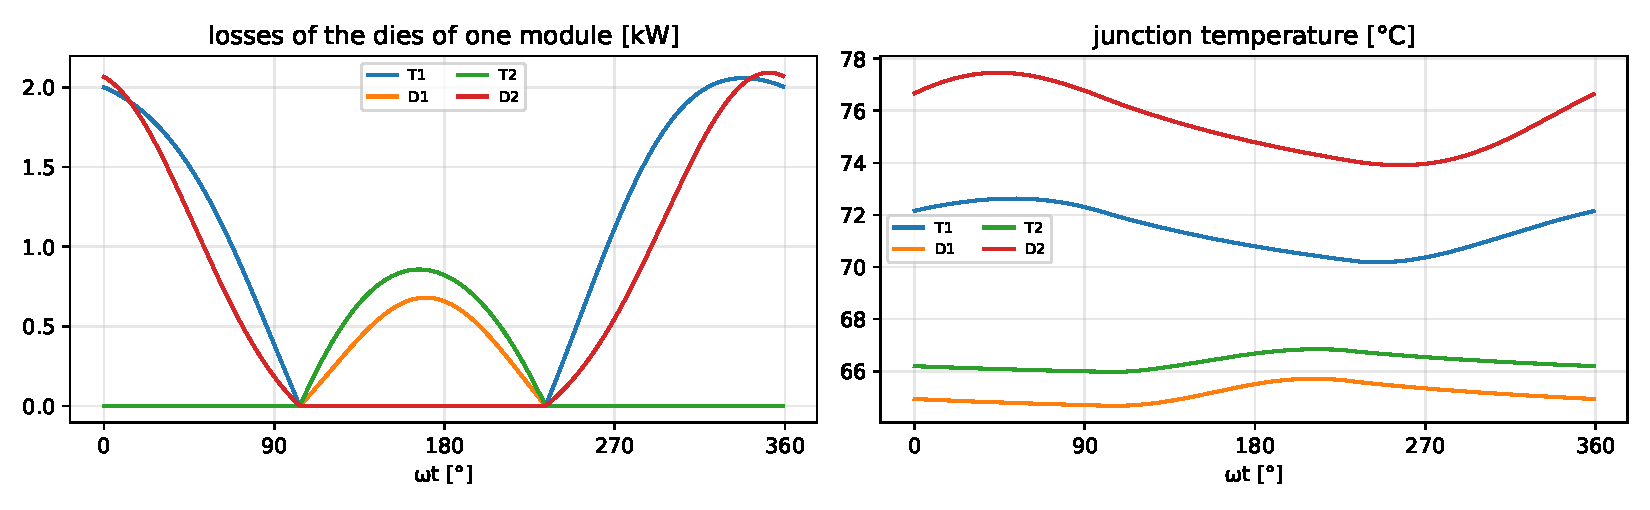
\includegraphics[width=\linewidth]{thermal/fig/junction_waveforms.pdf}
  \caption{Losses and junction temperatures of the dies over one period, example as in Table~\ref{tab:thermal-modules}}
  \label{fig:junction}
\end{figure}

Table~\ref{tab:thermal-flow} gives the highest junction temperature against the water flow per cold plate and the
inlet temperature. The inlet temperature adds one to one; halving the flow from 10\,l/min to 5\,l/min raises the
highest junction temperature by 8.3\,K.

\begin{table}[!ht]
  \centering
  \small
  \begin{tabular}{@{}r r r r@{}}
    \toprule
    \multicolumn{1}{c}{\textbf{$Q_w$ [l/min]}} & \multicolumn{1}{c}{\textbf{$T_{w\_in} = 40\,^{\circ}$C}}
      & \multicolumn{1}{c}{\textbf{50\,$^{\circ}$C}} & \multicolumn{1}{c}{\textbf{60\,$^{\circ}$C}} \\
    \midrule
    \tablerows{thermal/fig/flow_table}
    \bottomrule
  \end{tabular}
  \caption{Highest junction temperature in $^{\circ}$C against water flow per cold plate and inlet temperature}
  \label{tab:thermal-flow}
\end{table}
\FloatBarrier
